\chapter{Implémentation du système}
\chaptermark{Système}
\minitoc
\newpage

\section{Introduction}

Les transactions effectuées par les clients ont des informations importantes contenues dans les “label de transaction”. Par exemple, une transaction peut ressortir avec un label: “PAIEMENT PAR CARTE CARREFOUR DAC VL AMIENS 05/01” qui contient les informations comme le nom du détaillant Carrefour et la ville AMIENS. Par conséquent, si on sait qu'il n'y a qu’un seul carrefour à Amiens, grâce à l’algorithme de store locator, détaillé plus haut, cette transaction est identifiée. Maintenant dans le cas où le label de la transaction ne contient aucune information pertinente (ex: "59091383100 §§"), on aimerait quand même savoir l’origine de la transaction.
L'algorithme du Scoring nous permet donc d’affecter les transactions en cas de manque d'informations dans le label de transaction. L'algorithme analyse le comportement d'achat des clients au cours de  la même  journée pour décider si les transactions étaient dans le programme ou non. Enfin, à partir des algorithmes de machine learning on pourra appliquer des modèles capables d’affecter ces types de transaction au magasin correspondant.

\newpage
\section{Analyse de données}
\subsection{Informations sur la taille et les variables du jeu de donnée:}
\begin{figure}[h]
\begin{center}
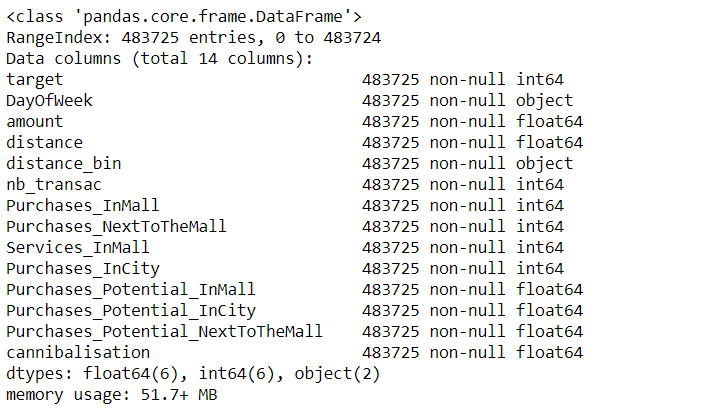
\includegraphics[width=15cm,height=8cm]{images/data_infos.png}
\caption[Informations sur la taille du jeu de donnée]{Informations sur la taille du jeu de donnée}
On distingue 3 types de variable dont 6 variables entiers, 6 float et 2 variables catégorielles.
\label{monlabel}
\end{center}
\end{figure}
\newpage

\subsection{Statistiques sur la dataset:}
\begin{figure}[h]
\begin{center}
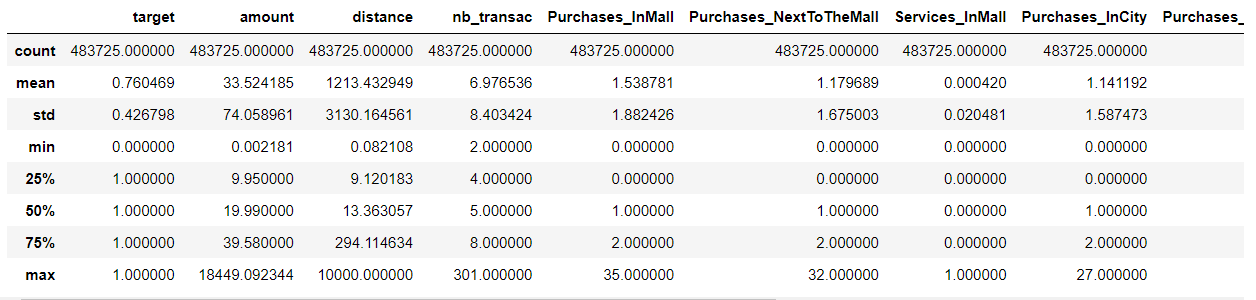
\includegraphics[width=15cm,height=4cm]{images/statistics_1.png}
\caption[Statistiques sur le jeu de donnée]{Statistiques sur le jeu de donnée}
\label{monlabel}
\end{center}
\end{figure}

\begin{figure}[h]
\begin{center}
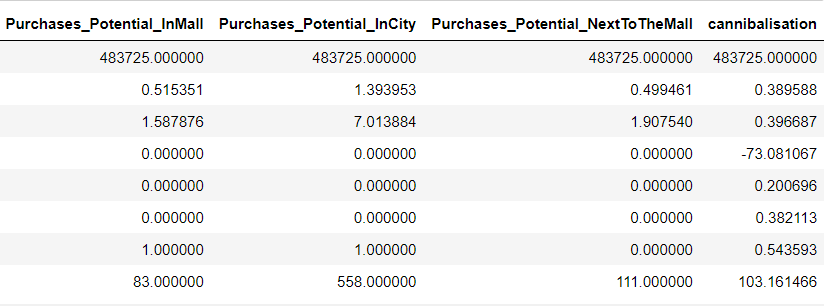
\includegraphics[width=15cm,height=4cm]{images/statistics_2.png}
\caption[Statistiques sur le jeu de donnée]{Statistiques sur le jeu de donnée}
\label{monlabel}
\end{center}
\end{figure}
\newpage

\subsection{Corrélation entre les variables numériques:}
\begin{figure}[h]
\begin{center}
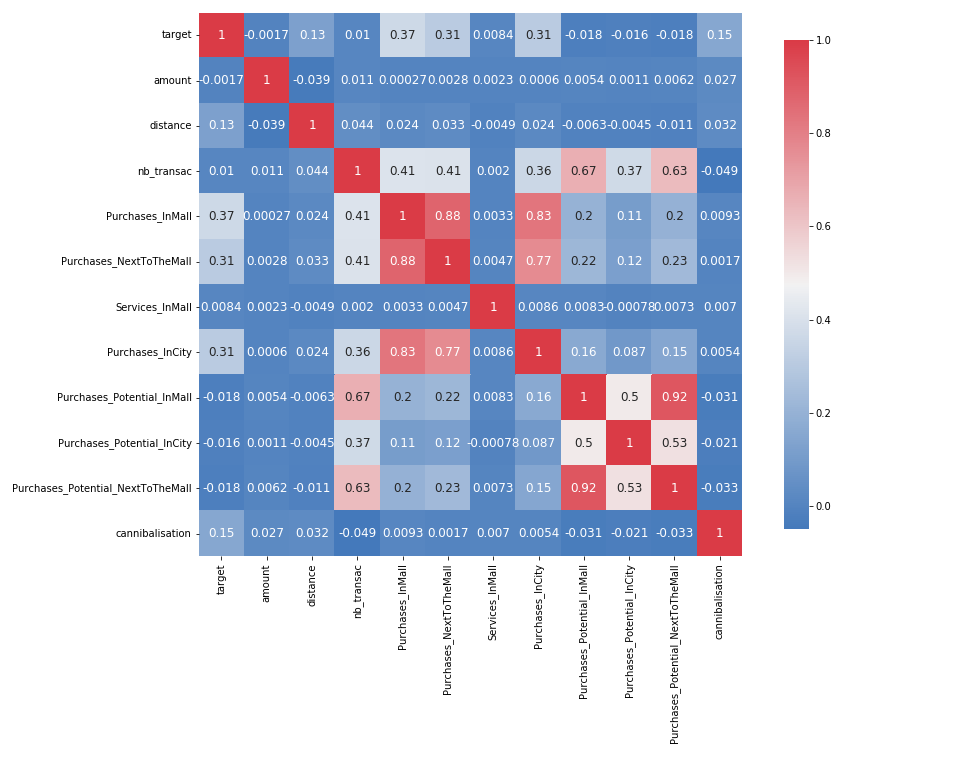
\includegraphics[width=18cm,height=12cm]{images/matrix_corelation.png}
\caption[Matrice de corrélation]{Matrice de corrélation}
\label{monlabel}
\end{center}
\end{figure}
On peut remarquer par exemple à partir de cette matrice de corrélation une forte liaison à 0.92 entre les variables Purchases-Potential-NextToTheMall et Purchases-Potential-InMall. Il est donc possible d’éliminer une de ces deux variables lors de la construction du modèle.

\newpage

\subsection{Relation entre les variables catégoriels:}
- Variable DayOfWeek:\\
\begin{figure}[h]
\begin{center}
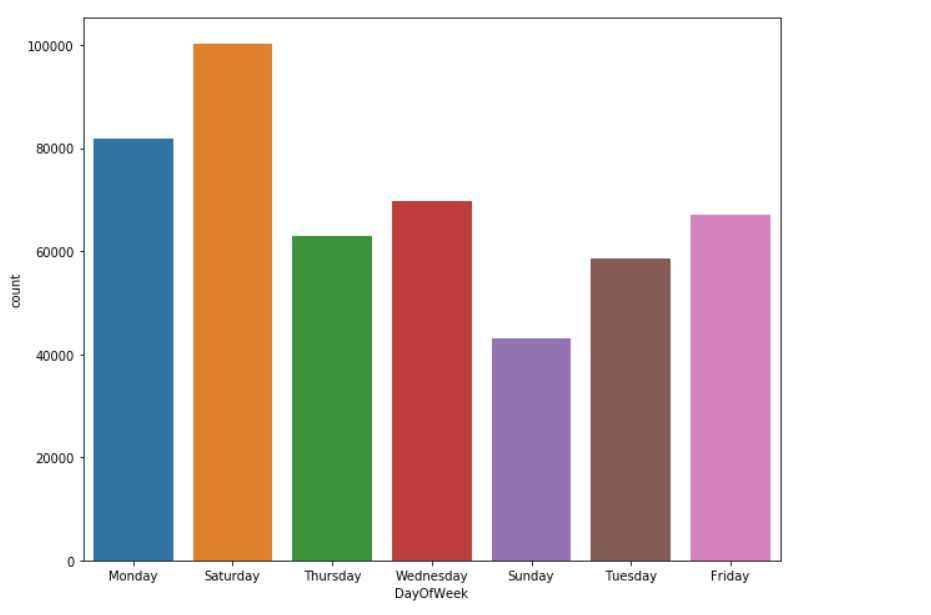
\includegraphics[width=15cm,height=6cm]{images/day_week.png}
\caption[Proportion des clients en fonction des jours]{Proportion des clients en fonction des jours}
\label{monlabel}
\end{center}
\end{figure}
On remarque que les clients ont naturellement tendance à effectuer des transactions le samedi puis le lundi que les autres jours. Ce qui rend cette variable importante dans la décision.

- Variable Distance-bin:\\
\begin{figure}[h]
\begin{center}
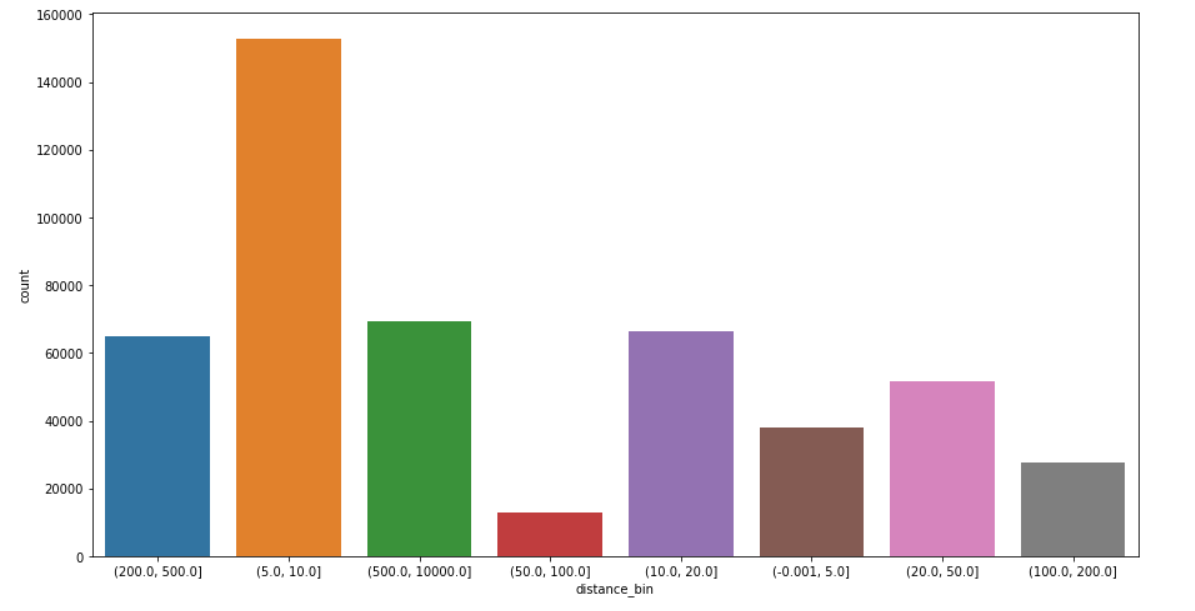
\includegraphics[width=15cm,height=6cm]{images/near_store.png}
\caption[Proportion des clients en fonction des jours]{Proportion des clients en fonction des jours}
\label{monlabel}
\end{center}
\end{figure}
La distance Bin ici constitue le magasin le plus proche du centre visité par le client. On remarque que la majorité des clients visitent d’autres magasins en dehors du centre entre 5 à 10 mètres.
\newpage

\section{Application des différents modèles au jeu de données}
\subsection{Résultats de l’application des modèles sur le jeu de donnée}
\begin{figure}[h]
\begin{center}
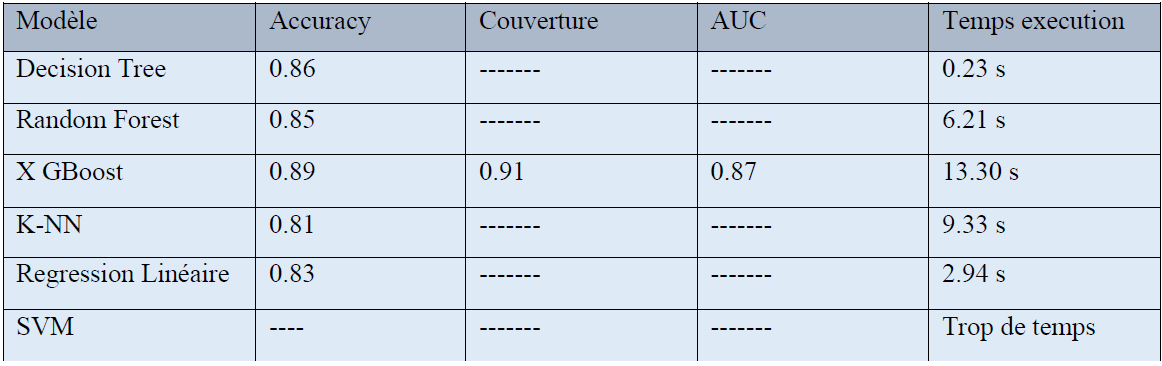
\includegraphics[width=15cm,height=6cm]{images/accuracy_modeles.png}
\caption[Statistiques d'apprentissage]{Statistiques d'apprentissage}
\label{monlabel}
\end{center}
\end{figure}

\begin{figure}[h]
\begin{center}
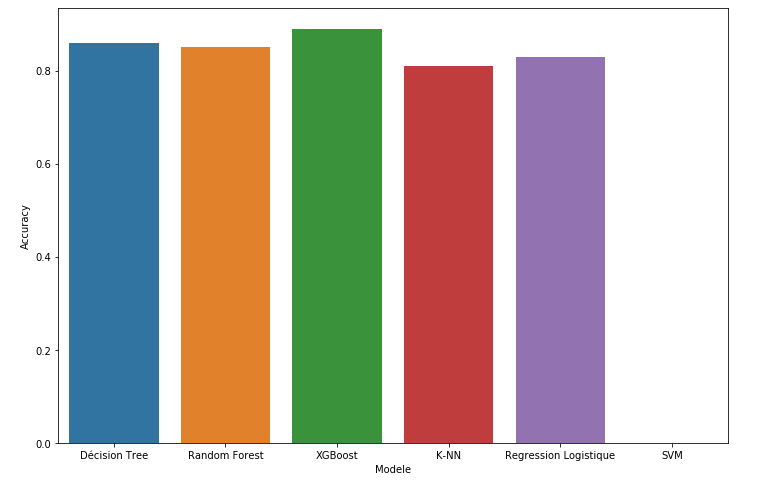
\includegraphics[width=15cm,height=6cm]{images/diagram_modeles.png}
\caption[Score des modèles]{Score des modèles}
\label{monlabel}
\end{center}
\end{figure}
A travers ces résultats on remarque que le modèle XGBoost est plus efficace en score que les autres modèles sur le jeu de données.

- Cas particulier du X GBoost:\\
L’avantage que présente XG Boost est qu’il donne en plus de la prédiction, la probabilité d’appartenance à chaque classe. Ce qui nous permet d’évaluer le taux de succès en fonction de la couverture de la prédiction sur le jeu de données.
\begin{figure}[h]
\begin{center}
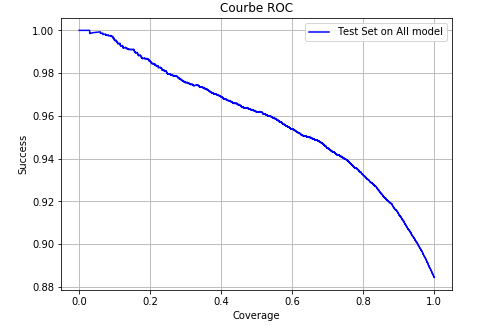
\includegraphics[width=15cm,height=9cm]{images/roc_auc.png}
\caption[Courbe de AUC]{Courbe de AUC}
\label{monlabel}
\end{center}
\end{figure}
\newpage

\subsection{Tests et validation: Matrice de Confusion}
Afin d’évaluer le taux d’erreur, on a essayé d’évaluer la matrice de confusion de chaque modèle. Sur la figure suivante seul le modèle XGBoost présente un faible taux de Faux Positif et de Vrai Négatif à 0.11. Ce qui rend ce modèle plus précis que les autres.
\begin{figure}[h]
\begin{center}
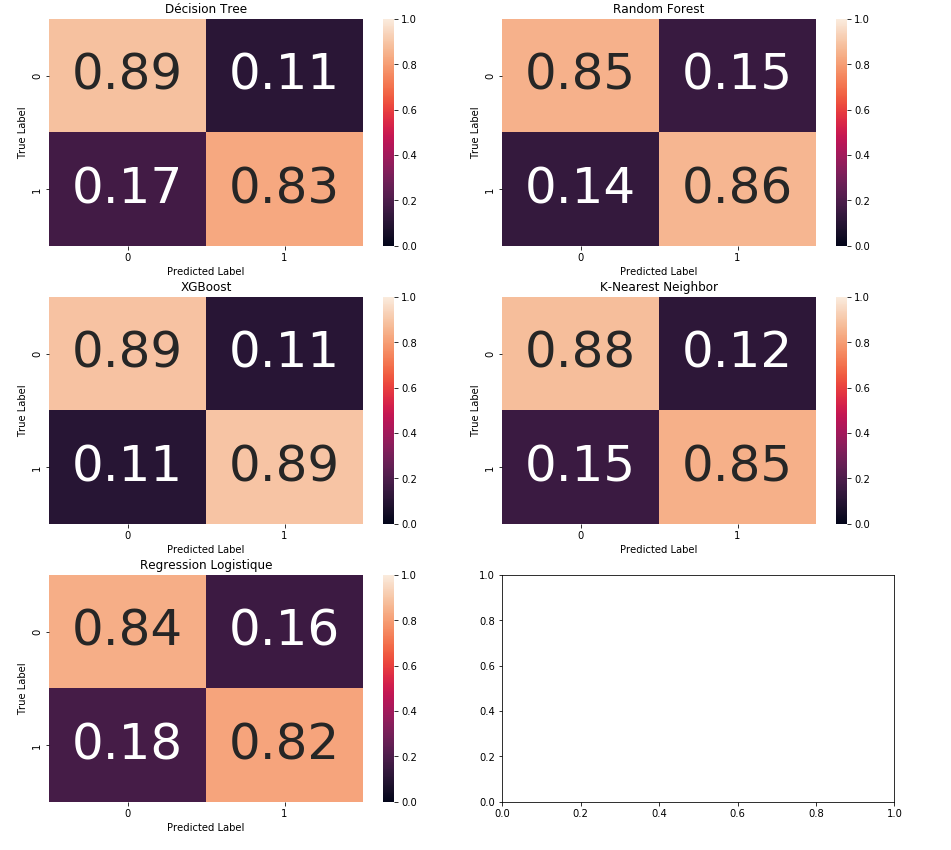
\includegraphics[width=15cm,height=14cm]{images/confusion_matrix.png}
\caption[Matrice de Confusion]{Matrice de Confusion}
\label{monlabel}
\end{center}
\end{figure}
\newpage

\section{Conclusion}
Au vu de tous ces résultats qui montrent la performance de XGBoost, on a décidé de choisir cette dernière comme modèle classification qui sera déployé en production. Des améliorations pourront éventuellement intervenir prochainement notamment au niveau du temps de calcul des variables. Dans quelques mois les données seront multipliées par deux et il sera nécessaire de passer de redshift vers peut être Spark afin de distribuer le calcul des variables. 